\documentclass[12pt]{article}
\usepackage[margin=1in]{geometry}
\usepackage {setspace} %% for line space
\usepackage[hang,flushmargin]{footmisc} %control footnote indent
\usepackage{url} % for website links
\usepackage{amssymb,amsmath}%for matrix
\usepackage{graphicx}%for figure
\usepackage{appendix}%for appendix
\usepackage{float}
\usepackage{multirow}
\usepackage{longtable}
\usepackage{morefloats}%in case there are too many float tables and figures
\usepackage{caption}
\usepackage{subcaption}
\usepackage{listings}
\captionsetup[subtable]{font=normal}
\usepackage{color}
\usepackage{hyperref}
\usepackage[utf8]{inputenc}

\setlength{\parindent}{0em}% paragraph indention
\setlength{\parskip}{0.5em}

\graphicspath{{figure/}}


\begin{document}
%\input{Proposal_draft-concordance}
%cover page
\begin{titlepage}
\title{\normalsize SEMIPARAMETRIC BAYESIAN LINEAR QUANTILE MIXED MODEL AND ITS APPLICATION}
\date{}
\maketitle

{\normalsize
\begin{center}
by\\[5mm]
Ming Yang, MS\\[10mm]
APPROVED:\\[10mm]
\end{center}}

\begin{table}[h]
\begin{flushright}
\begin{tabular}{ p{8cm}}

\hline
Stacia DeSantis, PHD\ \\[0.8cm]
\hline
Sheng Luo, PHD\\[0.8cm]
\hline
David R. Lairson, PHD\\[0.8cm]
\hline
Xiaoming Liu, PHD\\[0.8cm]


\end{tabular}
\end{flushright}
\label{default}
\end{table}

\thispagestyle{empty}
\pagestyle{empty}
\end{titlepage}

\newpage
\thispagestyle{empty}
\begin{center}
Coptyright\\
by\\
Ming Yang, MS\\
2014
\end{center}


\newpage
\thispagestyle{empty}
\doublespacing
\begin{center}
DEDICATION\\
xxx\\
xxx
\end{center}


\newpage
\thispagestyle{empty}
\doublespacing
\begin{center}
{\normalsize SEMIPARAMETRIC BAYESIAN LINEAR MIXED MODEL AND ITS APPLICATION}\\[3.2cm]

by\\[0.5cm]

Ming Yang, MS\\[3.2cm]

Presented to the Faculty of The University of Texas\\
School of Public Health\\
in Partial Fulfillment\\
of the Requirements\\
for the Degree of\\[1.5cm]
DOCTOR OF PHILOSOPHY\\[1.5cm]
\singlespacing
THE UNIVERSITY OF TEXAS\\
SCHOOL OF PULIC HEALTH\\
Houston, Texas\\
month, 2014
\end{center}


\newpage
\thispagestyle{empty}
\doublespacing
\begin{center}
ACKNOWLEDGEMENTS
\end{center}
text text text


\newpage
\thispagestyle{empty}
\doublespacing
\begin{center}
{\normalsize SEMIPARAMETRIC BAYESIAN LINEAR MIXED MODEL AND ITS APPLICATION}\\[2.3cm]
\singlespacing
Ming Yang, MS\\
The University of Texas\\
School of Public Health, 2014
\end{center}

\doublespacing
\noindent
Thesis Chair, Stacia DeSantis, PhD\\
\indent
text text text



\newpage
\tableofcontents

\newpage
\listoftables

\newpage
\listoffigures
 

\newpage
\section{Background}%%%%%%%%%%%%%%%%%%%%
\doublespacing
\indent Mixed effects model methodology, first introduced by R.A. Fisher \cite{fisher1919xv},  is a statistical tool that is used across a wide variety of disciplines including biostatistical contexts. Mixed effects models are especially popular in researches involving repeated measurements or observations from multilevel (or hierarchical) structure where the correlation between observations is not negligible. In the context of Bayesian data analysis for linear mixed models (LMM) or generalized linear models (GLMM), normal (or multivariate normal) distribution is a conventional prior for the random effects. However, the choice of normal prior is simply for mathematical convenience but without any theoretical justification.  Several studies have revealed that estimation for the fixed effects is relatively robust to the prior choice of the random effects \cite{neuhaus1992effects} \cite{butler1992random} \cite{kleinman1998semiparametric}, which suggests that the estimates for the fixed effects are asymptoticly valid even when the normal prior is not appropriate. However, in practice, inference on random effects may be also of interest, for example, the block random effects in randomized block designs. Accurate estimation of the random effects is especially important when we are trying to make predictions for some specific subject in the future. Since the estimate of the random effects is very sensitive to the choice of the prior and different priors will lead to totally different posterior distributions. In such cases, simply imposing normal prior to random effects is criticized for causing potential consequences, such as the results are sensitive to outliers \cite{dunson2010nonparametric}, less efficiency for non-normal data \cite{mehrotra1997non}, and the validity of the normality assumption is hard to assess since they are latent variables. In addition, we always would like to express our prior belief more accurately by choosing other distributions rather than blindly using normal in modeling the random effect. 

Some authors have proposed to use more flexible parametric alternatives than normal such as the heavier-tailed $t$ distribution and its skew extension \cite{lee2008flexible}. But these are still restrictive because they don't allow multi-modality in the data \cite{dunson2010nonparametric}. In handling all these problems at once, a Bayesian nonparametric method provides an ideal solution by using the Dirichlet process (DP) to replace the normal distribution as a much more flexible prior for random effects. In general, by using DP prior we model the distribution of the random effects with infinite mixture of distribution functions so that we capture the uncertainty and irregularity (outliers, skewness and clustering, etc.) in the data. More details about DP will be introduced in Section \ref{sec:DPM}. The performance of DP prior and normal prior will be compared using simulation study.\par

Quantile regression models are becoming more and more popular in the statistical community in recent years. Compared with the ubiquitous mean regression (a.n.a. linear regression) models, quantile regression models provide a much more comprehensive and focused insight into the association between the variables by studying the conditional quantiles functions of the outcome,  which may not be observed by looking only at conditional mean models \cite{koenker2005quantile}. In quantile regression, the regression coefficients (${\bf \beta}$) are functions of the quantile ($\tau$), and their estimates vary according to different quantiles. Thus quartile regression provides a way to studying the heterogeneity of the outcome that is associated with the covariates \cite{koenker2005quantile}. Moreover, quantile regression is more robust against outliers in the outcome compared with the mean regression, which is an immediate extension from the property of quantiles. \par


For a linear quantile regression model, \cite{koenker1978regression} introduced a method in estimating the conditional quantiles. As an introductory material, Koenker \cite{koenker2001quantile} briefly covers the fundamentals of quantile regression, parameter estimation techniques, inference, asymptotic theory, etc., his book \cite{koenker2005quantile} provides more comprehensive and deeper introduction on quantile regression related topics.  Yu and Moyeed \cite{yu2001bayesian} introduced the idea of Bayesian quantile regression by modeling the error term using asymmetric Laplace distribution (ALD) followed the idea proposed in \cite{koenker1978regression}. \cite{kozumi2011gibbs} developed a Gibbs sampling algorithm for Bayesian quantile regression models, in which they used a location-scale mixture representation of the ALD. Many works have been done to extend the quantile regression method to accommodate longitudinal data. \cite{jung1996quasi} developed a quansi-likehood method for median regression model for longitudinal data. \cite{geraci2007quantile} proposed to fit the quantile regression for longitudinal data based on ALD and the estimation is made by using Monte Carlo EM algorithm, later on \cite{liu2009mixed} followed the idea of \cite{geraci2007quantile} and extended the model from random intercept to include random regression coefficients as well. \cite{fu2012quantile} proposed  a working correlation model for quantile regression for longitudinal data, a induced smoothing method was used to make the inference of the estimators. Fully Bayesian techniques were also developed for fitting linear quantile mixed models, for example \cite{luo2012bayesian} used the similar idea as \cite{kozumi2011gibbs} did in decomposing the error term as a location-scale mixture and developed a Gibbs sampling algorithm for quantile linear mixed model. The fully Bayesian method is appealing because it is easy to implement and to make inference, the uncertainty of the unknowns is taken into account, and it is flexible in the distribution of random effects. The detailed background about Bayesian quantile linear mixed model will be introduced in Section \ref{sec:BLQMM}. In addition, temporal\par

A novel idea that combines the linear quantile mixed model and nonparametric Bayesian methodology in studying the longitudinal data can be an important supplement to existing methods. Longitudinal or correlated data commonly arise in biostatistical context. For example, they can be measurements that are taken repeatedly over time, or outcomes from grouped patients in clinical trials. Moreover, real data can be far from ideal situation, which means extreme observations can be possibly included. It is crucial that a proper method to be used in order to make a better investigation of the relationship between the outcome of interest and potential risk factors. Traditional mean regression model is easy to grasp and implement, but it also suffers from its fragility in facing of the outliers. Ignoring the outliers in analysis could lead to misleading conclusion \cite{koenker2001quantile}. The quantile regression method can be a sensible supplement where the mean regression shouldn't be used in those situations. \par

\emph{[Add background for topic two here.]}\par

To sum up, this research project focuses on developing and applying new statistical methods in analysis longitudinal data and will cover the following topics. First, a statistical method that combines nonparametric Bayesian technique and the quartile regression model in analyzing longitudinal data will be introduced. In this part, the linear quantile mixed model is used so that the within subject correlation is accounted and the results also will be more robust to potential outlying observations. Since we used quantile regress instead of mean regression, a more comprehensive insight about the association between the outcome and covariates will be learned. As mentioned, in this part we will use DP to model the random effects in linear quantile mixed model, which is robust to the true underlying distribution of random effects and supposed to provide better prediction of the random effects. Second, as studying the temporal data, we will focus on the prediction of future outcomes. \par



\section{Specific Aims and Hypotheses}%%%%%%%%%%%%%%%%%%%%

\begin{enumerate}
\item To incorporate nonparametric Bayesian method with quantile linear mixed model to analyze longitudinal data.

\item To obtain accurate prediction of the random effects in mixed model so that accurate prediction for future outcomes can be made. When given new covariates ${\bf x}_0$, the posterior predictive density of future outcome, given observed values, is formulated as
\begin{eqnarray}\label{eqn:ppv}
r(\tilde{y}|{\bf y})&=&\int g(\tilde{y}, \boldsymbol{\theta}|{\bf y})d\boldsymbol{\theta}=\int q(\tilde{y}|\boldsymbol{\theta})p(\boldsymbol{\theta}|{\bf y})d\boldsymbol{\theta},
\end{eqnarray}
where $\boldsymbol{\theta}$ are the posterior samples from MCMC iterations.
\end{enumerate}


\section{Data}%%%%%%%%%%%%%%%%%%%%
Traumatic brain injury (TBI) data.

\section{Methods}%%%%%%%%%%%%%%%%%%%%

\subsection{Nonparametric Bayesian}%%%%%%%%%%%%%%%%%%%%%%%%%%%%%%%%%%%%%%%%

\subsubsection{Dirichlet Process and Dirichlet Process Mixture Models}\label{sec:DPM}%%%%
A {\em Dirichlet process} (DP), first introduced by Ferguson in 1973 \cite{ferguson1973bayesian}, is a random probability model (RPM), is a probability distribution whose domain is itself a set of probability distributions. A Dirichlet process, denoted by DP$\left(\alpha, H\right)$,  is specified by two parameters: the concentration parameter $\alpha$, which is a positive real number and the base distribution (or base measure) $H$ that is an arbitrary distribution. A draw from DP will return a random distribution (the output distribution) over some some probability space $\Theta$ that can be drawn from $H$. Let $A_1,\cdots, A_r$ be any finite partition of the probability space $\Theta$, then we say the RPM $G$ is a a Dirichlet process with base measure $H$ and concentration parameter $\alpha$ if 
\begin{equation}\label{eqn:dir_dist}
(G(A_1), \cdots, G(A_r))\sim Dir(\alpha H(A_1), \cdots, \alpha H(A_r))
\end{equation}

An intuitive understanding of Equation (\ref{eqn:dir_dist}) is that the concentration parameter $\alpha$ defines the inverse variance of DP as $Var(G(A))=H(A)(1-H(A))/(\alpha+1)$ while the base distribution defines the mean of DP: $E(G(A))=H(A)$. Larger $\alpha$ leads to smaller variance of DP and as a result, it will concentrate more around its mean. Consequently, as $\alpha\rightarrow\infty$, we have $G(A)\rightarrow H(A)$ \cite{ferguson1973bayesian}. 


Regarding the computational purpose, there are different realization methods for DP and here we only mention two of them. The first is the P\'{o}lya urn scheme \cite{blackwell1973ferguson}, which is formulated as follows 
\begin{eqnarray}\label{eqn:polya}
&& \theta_i|G\overset{iid}\sim G, \mbox{ for } i=1,2, \cdots, \mbox{ where} \nonumber\\
&& G\sim DP(\alpha, H)\\
&& \theta_1\sim H, \mbox{ and } \theta_{n+1}|\theta_1,\cdots, \theta_n\sim\frac{1}{\alpha+n}\left(\alpha H+\sum_{i=1}^n\delta_{\theta_i}\right).\nonumber
\end{eqnarray}

\noindent The other is the stick-breaking representation \cite{sethuraman1991constructive}:
\begin{eqnarray}\label{eqn:sb}
&& \theta_i|G\overset{iid}\sim G\mbox{ for } i=1,2, \cdots , \mbox{ where}\nonumber\\
&& G\sim DP(\alpha, H)\\
&& G=\sum_{i=1}^{\infty} V_i\prod_{l<i}(1-V_l)\delta_{\theta_i} \mbox{ with } V_i\overset{iid}\sim Beta(1,\alpha)\mbox{ and }\theta_i\overset{iid}\sim H.\nonumber
\end{eqnarray}

\noindent where in both representations $\delta_{\theta_i}$ is the point mass at $\theta_i$. Due to its simplicity, using the stick-breaking structure,  with a selection of appropriate priors for the hyper-parameters for parameters in (\ref{eqn:sb}), a fully Bayesian algorithm is easy to develop and implement, and inference for DPM models can be made from MCMC simulation.\par

\noindent From (\ref{eqn:sb}) we can see that the DP is just a infinite mixtures of point masses, which include infinitely many parameters. And although the base distribution $H$ is continuous, the DP is almost surely discrete. The discreteness property of DP limits its applications to many problems where the distribution to model is believed to be continuous. To overcome this constraint, a simple extension was developed by introducing additional convolution:

\begin{eqnarray}\label{eqn:dpm}
&& \theta_i|\boldsymbol{\eta}_{k} \sim f(\cdot|\boldsymbol{\eta}_k), \ k=1, 2, \cdots\\
&& \boldsymbol{\eta}_k|G\overset{iid}\sim G,\  G\sim DP(\alpha, H)\nonumber
\end{eqnarray}

\noindent where $f(\cdot)$ is a continuous density function (usually is normal distribution) for $\theta_i$ with parameter $\boldsymbol{\eta}$ and  as a result, $\theta_i\sim\sum_{k=1}^{\infty}w_kf(\cdot|\boldsymbol{\eta}_k)$, where $w_k=V_k\prod_{l<k}(1-V_l)$. This model is referred as Dirichlet process mixture (DPM) model\cite{escobar1995bayesian}. 


\subsubsection{Centered Dirichlet Process Mixture}\label{sec:DPM}%%%%
In statistical modeling, the parameter $\theta$ (in some parameter space $\Theta$) in the probability distribution $\mathcal{P}_\theta$ is not identifiable if and only if there is another parameter $\theta^*\in \Theta$, with $\theta^*\ne\theta$ and $\mathcal{P}_{\theta}=\mathcal{P}_{\theta^*}$. In linear mixed models, i.e. $y_{ij}=\beta_0+\boldsymbol{\beta}'{\bf X}_{ij}+\theta_i+\varepsilon_{ij}$, with $E(y_{ij})=\beta_0+\boldsymbol{\beta}'{\bf X}_{ij}+\mu_{\theta_i}$, to avoid the identifiability problem of the regression intercept and mean parameter of the random effects, people usually constrain the normal prior to have mean zero with some variance parameter. Similar problem also occur when we use the DPM prior for the random effects, since mean of the mixture distribute is not zero by default in (\ref{eqn:dpm}). To work around the identifiability problem, \cite{yang2010semiparametric} proposed a revised stick-breaking procedure that standardizes the random samples from DPM to make its mean be zero and the resulting DPM model is named centered DPM (CDPM) model. Take the mixtures of normal model as an example, the procedure is done as follows:

\begin{eqnarray}\label{eqn:cdpm}
&& \boldsymbol (\boldsymbol{\mu}_k, \boldsymbol{\Sigma}_k)|G\overset{iid}\sim G,\ k=1,2,\cdots\nonumber\\
&& \boldsymbol{\mu}^*_k=\boldsymbol{\mu}_k-\sum_{i=k}^{\infty}w_k\boldsymbol{\mu}_k , \mbox{ with } w_k=V_k\prod_{l<k}(1-V_l),V_k\overset{iid}\sim Beta(1,\alpha)\\
&& \boldsymbol{\theta}_i|\boldsymbol{\mu}^*_k, \boldsymbol{\Sigma}_k\sim N(\boldsymbol{\mu}^*_k, \boldsymbol{\Sigma}_k)\nonumber
\end{eqnarray}


\subsubsection{Truncation}\label{sec:tru}%%%%
However, it is impossible to get exact samples from a DP since it needs to perform draws from an infinitely many mixtures of densities. By noticing that the random weights $w_i$ assigned to the densities decrease as the number of mixture index $i$ increases, some authors proposed a strategy to bypass this issue by choosing a large enough $N$ for mixture to approximate the full DPM \cite{muliere1998approximating} \cite{ishwaran2001gibbs} \cite{kottas2001bayesian} \cite{ohlssen2007flexible}, i.e.

\begin{equation}\label{eqn:trun}
G^*=\sum_{k=1}^N w_kf(\cdot)
\end{equation}

In \cite{ishwaran2000inference}, Ishwaran gives some theoretical comparison to assess the difference between truncated DP and full DP under the setting of generalized linear mixed models. He also proposed a blocked Gibbs sampler based on the truncation of the stick-breaking representation. Based on Ishwaran's theory, if we choose $N=200$ and $\alpha=10$, the loss of the approximation by truncation is negligible ($\le 9.1e^{-7}$). In our application, we will compare the performance of truncated DPM for different values of $N$.


\subsection{Linear Quantile Mixed Models}\label{sec:QMM}%%%%%

\subsubsection{Quantile Regression and Asymmetric Laplace Distribution}\label{sec:QRALD}%%%%%

Let $Y$ be a real valued random variable with cumulative distribution function $F_Y(y) = P(Y \le y)$. The $\tau^{th}$ quantile of $Y$, where $\tau\in[0,1]$,  is given by
\begin{equation}\label{eqn:quantile}
Q_{Y}(\tau)=F_{Y}^{-1}(\tau)=\inf\left\{ y:F_{Y}(y)\geq\tau\right\}
\end{equation}

In quantile regression context, similar as in linear regression, the conditional quantile of $Y$ is model as a linear function of other covariate, which is defined as

\begin{equation}\label{eqn:lqr}
Q_{y|{\bf x}}(\tau)={\bf x}^{T}\boldsymbol{\beta}_{\tau}
\end{equation}

Given the data sample, the estimates of the regression coefficients at $\tau^{th}$ quantile can be obtained by solving 

\begin{equation}\label{eqn:loss_fun}
\hat{\boldsymbol{\beta}}_{\tau}=\underset{\boldsymbol{\beta}\in \mathbb{R}^{p}}{\mbox{arg min}}\sum_{i=1}^{n}\left[\rho_{\tau}(y_{i}-{\bf x}_i^{T}\boldsymbol{\beta})\right],
\end{equation}

where the loss function $\rho_{\tau}(\cdot)$ is defined as $\rho_{\tau}(y)=y(\tau-{I}{(y<0)}).$ \par

\noindent There is not direct solution to solve (\ref{eqn:loss_fun}) rather the minimization problem can be reformulated as a linear programming problem, where simplex methods or interior point methods can be applied to solve for the estimates \cite{koenker2005quantile}. The minimization problem can also be rephrased as a maximum-likelihood problem by using the asymmetrical Laplace distribution (ALD). \cite{koenker1999goodness} \cite{yu2001bayesian}.

Suppose a random variable $Y$ follows ALD($\mu, \sigma, \tau$), then the probability density function of $Y$ can be written as

\begin{equation}\label{eqn:ald}
f(y|\mu, \sigma, \tau)=\frac{\tau(1-\tau)}{\sigma}\exp\left[-\rho_{\tau}\left(\frac{y-\mu}{\sigma}\right)\right],
\end{equation}

where $\mu\in(-\infty, \infty)$ is the location parameter, $\sigma$ is the scale parameter and $\tau\in(0, 1)$ is the skewness parameter. Thus, in a standard linear model

\begin{equation}\label{eqn:lm}
y_i={\bf x_i}^{T}\boldsymbol{\beta}+\varepsilon_i,
\end{equation}

if we assume the random error $\varepsilon_i\sim$ ALD($0, \sigma, \tau$), then $y_i|{\bf x}_i\sim$
ALD(${\bf x_i}^{T}\boldsymbol{\beta}, \sigma, \tau$), that is the likelihood function can be written as

\begin{equation}\label{eqn:yald}
L(\boldsymbol{\beta}, \sigma; {\bf y}, \tau)\propto\frac{1}{\sigma^n}\exp\left[-\sum_{i=1}^n\rho_{\tau}\left(\frac{y_i-{\bf x_i}^{T}\boldsymbol{\beta}}{\sigma}\right)\right].
\end{equation}

If we treat $\sigma$ in (\ref{eqn:yald}) as nuisance then the maximization of (\ref{eqn:yald}) with respect to $\boldsymbol{\beta}$ is exactly the same as that in (\ref{eqn:loss_fun}).



\subsubsection{Bayesian Linear Quantile Mixed Model}\label{sec:BLQMM}%%%%%

Linear quantile mixed model (LQMM) is defined as
\begin{equation}\label{eqn:lqmm}
Q_{y_{ij}|{\bf x}_{ij}}(\tau)={\bf x}_{ij}^{T}\boldsymbol{\beta} + {\bf z}_{ij}^{T}\boldsymbol{\alpha}_i,\ i=1, \cdots, N,\ j=1,\cdots, n_i.
\end{equation}
where $y_{ij}$ is the response variable for subject $i$ at time $j$, ${\bf x}_{ij}$ is the $p-$dimensional fixed effects covariates and $\boldsymbol{\beta}_{\tau}$ is the corresponding $p\times1$ vector of fixed effects, while ${\bf z}_{ij}$ is the $k-$dimensional random effects covariates and $\boldsymbol{\alpha}_i$ is the corresponding $k\times 1$ vector of random effects. Under the assumption that the random error follows ALD$(0, \sigma, \tau)$ distribution, conditional on the random effects $\boldsymbol{\alpha}_i$, $y_{ij}$'s are independently and identically distributed as ALD(${\bf x}_{ij}'\boldsymbol{\beta}+{\bf z}_{ij}'\boldsymbol{\alpha}_i, \sigma, \tau$):

\begin{equation}\label{eqn:ald_lqmm}
f(y_{ij}|\boldsymbol{\beta},\boldsymbol{\alpha}_i,\sigma)=\frac{\tau(1-\tau)}{\sigma}\exp\left[-\rho_{\tau}\left(\frac{y_{ij}-{\bf x}_{ij}'\boldsymbol{\beta}-{\bf z}_{ij}'\boldsymbol{\alpha}_i}{\sigma}\right)\right]
\end{equation}

To develop a Gibbs sampler for model (\ref{eqn:ald_lqmm}), we need to assume a location-scale mixture representation of the ALD \cite{kotz2001laplace}. Under this assumption the random error is represented as $\varepsilon_{ij}=\gamma_1e_{ij}+\gamma_2\sqrt{\sigma e_{ij}}u_{ij}$,

where \[\gamma_1=\frac{1-2\tau}{\tau(1-\tau)}, \mbox{ and } \gamma_2^2=\frac{2}{\tau(1-\tau)},\]
and \[u_{ij}\sim N(0,1), \mbox{ and } e_{ij}\sim\exp(\sigma).\]

The linear mixed model is then reparameterized as
\begin{equation}\label{eqn:reformald2}
y_{ij}={\bf x}_{ij}'\boldsymbol{\beta}+{\bf z}_{ij}'\boldsymbol{\alpha}_i+\gamma_1e_{ij}+\gamma_2\sqrt{\sigma e_{ij}}u_{ij},
\end{equation}


or equivalently
\begin{equation}\label{eqn:lo_sc_lh}
f(y_{ij}|\boldsymbol{\beta},\boldsymbol{\alpha}_i,e_{ij},\sigma)=\frac{1}{\sqrt{2\pi\gamma_2^2\sigma e_{ij}}}\exp\left[-\frac{1}{2\gamma_2^2\sigma e_{ij}}(y_{ij}-{\bf x}_{ij}^{T}\boldsymbol{\beta}-{\bf z}_{ij}^{T}\boldsymbol{\alpha}_i-\gamma_1e_{ij})^2\right].
\end{equation}


Following (\ref{eqn:reformald2}), a fully specified Bayesian model would include follows:

\begin{eqnarray*}
&& {\bf u}\sim\prod_{i=1}^N\prod_{j=1}^{n_i}\exp\left(-\frac{u_{ij}^2}{2}\right)\\
&& {\bf e}\sim\prod_{i=1}^N\prod_{j=1}^{n_i}\frac{1}{\sigma}\exp\left(-\frac{e_{ij}}{\sigma}\right)\\
&& \boldsymbol{\beta} \sim MVN_p({\bf 0}, \boldsymbol{\Sigma})\\
&& \boldsymbol{\alpha}_i|\upsilon \sim MVN_p({\bf 0}, \upsilon^2\boldsymbol{I})\mbox{ or } \boldsymbol{\alpha}_i|G\sim DP(\alpha_0, H)\\
&& \sigma\sim IG(a_0, b_0)\\
&& \upsilon\sim IG(c_0, d_0)\mbox{ or }\alpha_0\sim IG(e_0, f_0), H\sim N(\mu_0, \sigma_0).
\end{eqnarray*}



\section{Plan for Simulation Studies}%%%%%%%%%

\subsection{Bayesian Quantile Regression Method}%%%%%%%%%
In this section, the simulation study will focus on fitting the Bayesian quantile linear mixed model (BLQMM) by using the ALD representation for the random errors. The focus will be checking the performance of the BLQMM method in estimating the regression coefficients. Here we will use the normal distribution as the prior for the random effects.

We simulate data from the model \begin{equation}\label{sim2}y_{ij}={\bf x}_{ij}'\boldsymbol{\beta}+{\bf z}_{ij}'\boldsymbol{\alpha}_i+(1+\gamma x_{ij})\varepsilon_{ij}\end{equation}
where the covariates $x_{ij}$ not only affects the location of $y_{ij}$ but also its scale,which is one of the reasons why we prefer to use quantile regression for such data. Based on equation (\ref{sim2}), the settings are similar to strategy one for the fixed and random effects and $\gamma$ is a parameter chosen for the heteroscedasticity of the data \cite{reed2009partially}. When $\gamma=0$, (\ref{sim2}) reduces to 

\begin{equation}\label{eqn:sim1} 
y_{ij}={\bf x}_{ij}'\boldsymbol{\beta}+{\bf z}_{ij}'\boldsymbol{\alpha}_i+\varepsilon_{ij}.\end{equation} 

Based on equation (\ref{sim2}), for a simplified model 
\begin{equation}\label{eqn3} 
y_{ij}=\beta_0+\beta_1*x_{ij}+\alpha_i+ (1+\gamma x_{ij})\varepsilon_{ij}
\end{equation}

The simulation study is carried out as follows: generate data from euqation (\ref{eqn3}), where \[\beta_0=10,\ \beta_1=-1,\ \gamma=1/11\]
\[x_{ij}\sim unif(0,10),\ \alpha_i\sim N(0,1),\ \varepsilon_{ij}\sim N(0,1)\] 

 Given $\boldsymbol{\beta}$ and $\tau$, the true values of $\tau^{th}$ quantile regression coefficients are given by 
\[{\beta}_0(\tau)=\beta_0+q_{\tau}(\varepsilon_i),\] 
\[\beta_1(\tau)=\beta_1+\gamma q_{\tau}(\varepsilon_i).\]
The Gibbs developed in Section \ref{sec:BLQMM} will be implement using \verb'Jags' and the inferno will be made based on the MCMC samples. The simulation results will be shown as follows

\begin{table}[H]
\caption{Simulation study with 500 datasets, $N(0,1)$ for error term}
\centering
\begin{tabular}{lcc}
\hline
$\tau=0.05$&$bias$&$RMSE$\\
\hline
$\beta_0(8.355)$& -0.0387 & 2.089 \\
$\beta_1(-1.150)$& 0.0754 & 0.118 \\
\hline
\hline
$\tau=0.25$&&\\
$\beta_0(9.326)$& -0.0300 & 1.049 \\
$\beta_1(-1.061)$& 0.0214 & 0.085 \\
\hline
\hline
$\tau=0.5$&&\\
$\beta_0(10)$& -0.0039 & 0.354 \\
$\beta_1(-1)$& 0.0078 & 0.071\\
\hline
\hline
$\tau=0.75$&&\\
$\beta_0(10.674)$& 0.0243 & 0.992 \\
$\beta_1(-0.939)$& -0.0096 & 0.089 \\
\hline
\hline
$\tau=0.95$&&\\
$\beta_0(11.644)$& 0.0374 & 2.070 \\
$\beta_1(-0.850)$& -0.0707 & 0.117 \\
\hline
\end{tabular}
\end{table}

%\subsubsection*{Comments}
%This is similar to what was done in \cite{luo2012bayesian} for the Table 1, the true value of the parameters were calculated the same way (confirmed). The original paper \cite{reed2009partially} did the simulation based on data generated from simple linear model in stead of linear mixed model though.


\subsection{Dirichlet Process Mixture Prior for Random Effects}%%%%
In this section of simulation study we aim to compare the performance of different prior distributions in modeling the random effects. We will investigate the effects of various priors on estimating the fixed and predicting the random effect with emphasis on random effects prediction. Estimation bias and credible interval will be calculated for the fixed effects for different prior assignments.  Regrading comparing the predicted random effects we will compare with respect to (a) estimating the true underlying distribution of the random effects, (b) the sums of squared difference between predicted versus generated random effects and (c) the posterior predictive values of the outcome based on the predicted random effects from different models.

The prior distributions under comparison include Gaussian (conventional one), $t$ distribution (heavier-tailed), and nonparametric Bayesian ones (DPM, CDPM). And the true underlying random effects are generated from Gaussian or non-Gaussian distributions like $t$ distribution (heavy tail), $Beta$ distribution (positively skewed) , and mixture of normals (multimodal).   \par


\subsubsection{Estimation of Fixed Effects}%%%%

Datasets will be simulated from the following formula with constant intercept 

\begin{equation}\label{eqn:sim_model2} 
y_{ij}=\beta_0+{\bf x}_{ij}'\boldsymbol{\beta}+\alpha_i+\varepsilon_{ij}
\end{equation}


\begin{table}[H]
\begin{center}
\caption{Sample summary table: estimation of fixed effects when $u_i\sim$ mixture Normal}
\begin{tabular}{cccccccccc}
\hline
&  & \multicolumn{2}{c}{\emph{Normal}} && \multicolumn{2}{c}{\emph{DPM}} & &\multicolumn{2}{c}{\emph{CDPM}} \\
\cline{3-4}\cline{6-7}\cline{9-10}
\emph{par}& \emph{truth}& \emph{est}    & \emph{95\% CI} & & \emph{est.}    & \emph{95\% CI}  && \emph{est.} & \emph{95\% CI}\\
\hline
$\beta_1$ & 1 & 0.929 &(0.775, 1.089)& &0.793 & (-0.357,1.803)& & 0.928&(0.820,1.037)\\
$\beta_2$ & 1 & 1.016&(0.963, 1.067) & & 1.017& (0.965,1.069)& &1.017 &(0.966,1.067)\\
$\beta_3$ & -1 & -0.957&(-1.007, -0.907) & & -0.957& (-1.010,-0.906)& &-0.956 &(-1.008,-0.905)\\
\hline
\end{tabular}
\end{center}
\end{table}





\subsubsection{Prediction of Random Effects}%%%%



\subsubsection*{Prediction of the distribution of random effects}%%%%

To compare the performance of DPM and conventional normal prior we simulated data based on Equation (\ref{eqn:sim1}), specifically,
\[\boldsymbol{\beta}=(1,1,-1)',\]
\[{\bf x}_{ij}=(x_{2ij}, x_{3ij})'\sim N_2\left({0 \choose 0},{\bf I}\right),\]
\[\varepsilon_{ij}\sim N(0,1).\] 

${\bf x_{1ij}}$ is a vector of 1's and simulate $\alpha_i$ from following different distributions respectively. We fit the simulated data with normal prior and DPPM for the random effect and compare the results by plotting them against the empirical data density of the random effect.

\begin{figure}[H]
\begin{minipage}{0.5\textwidth}
\centering
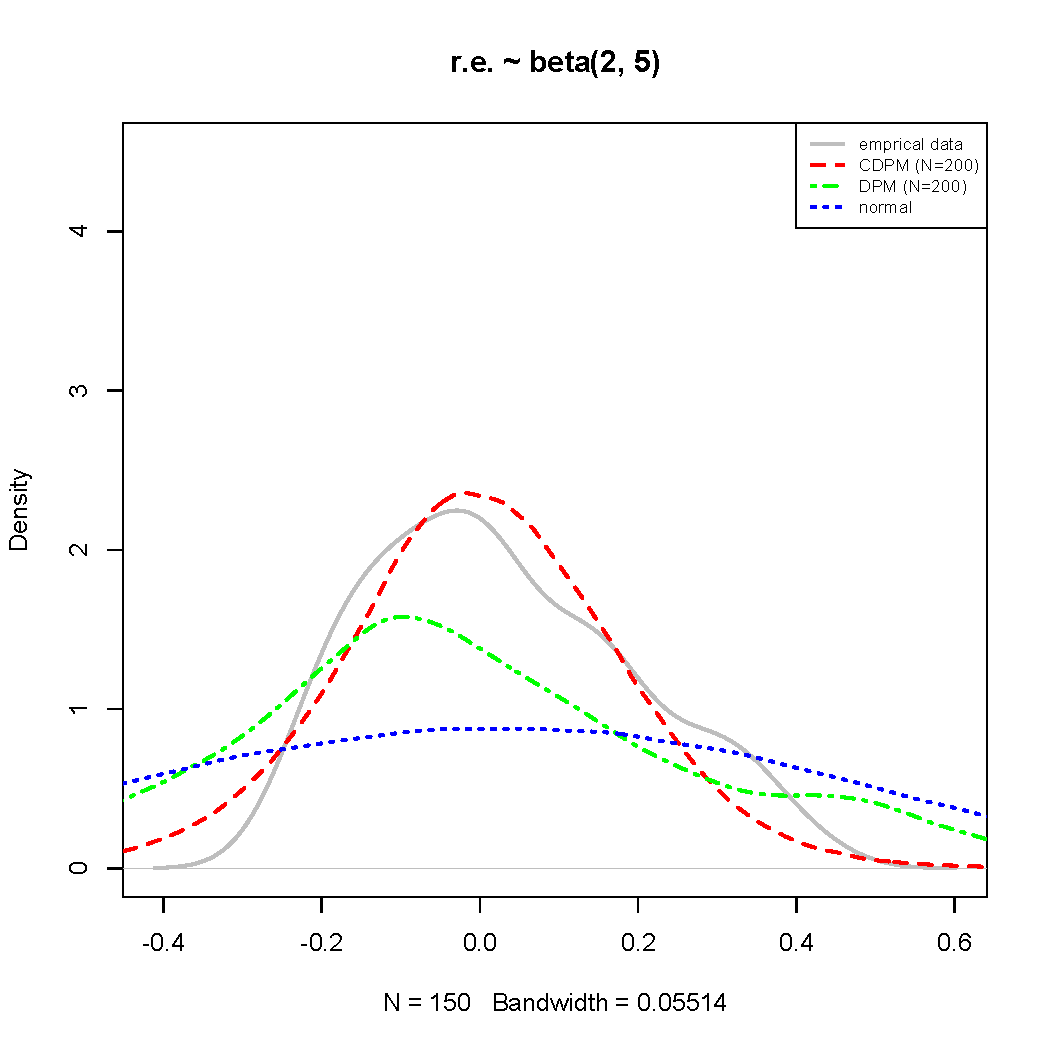
\includegraphics[width=0.85\textwidth]{ui_beta.pdf}
\label{fig: normal_dpm}
\caption{\small Predicted densities of random effects that follow beta distribution}
\end{minipage}
\hspace{0.5cm}
\begin{minipage}{0.5\textwidth}
\centering
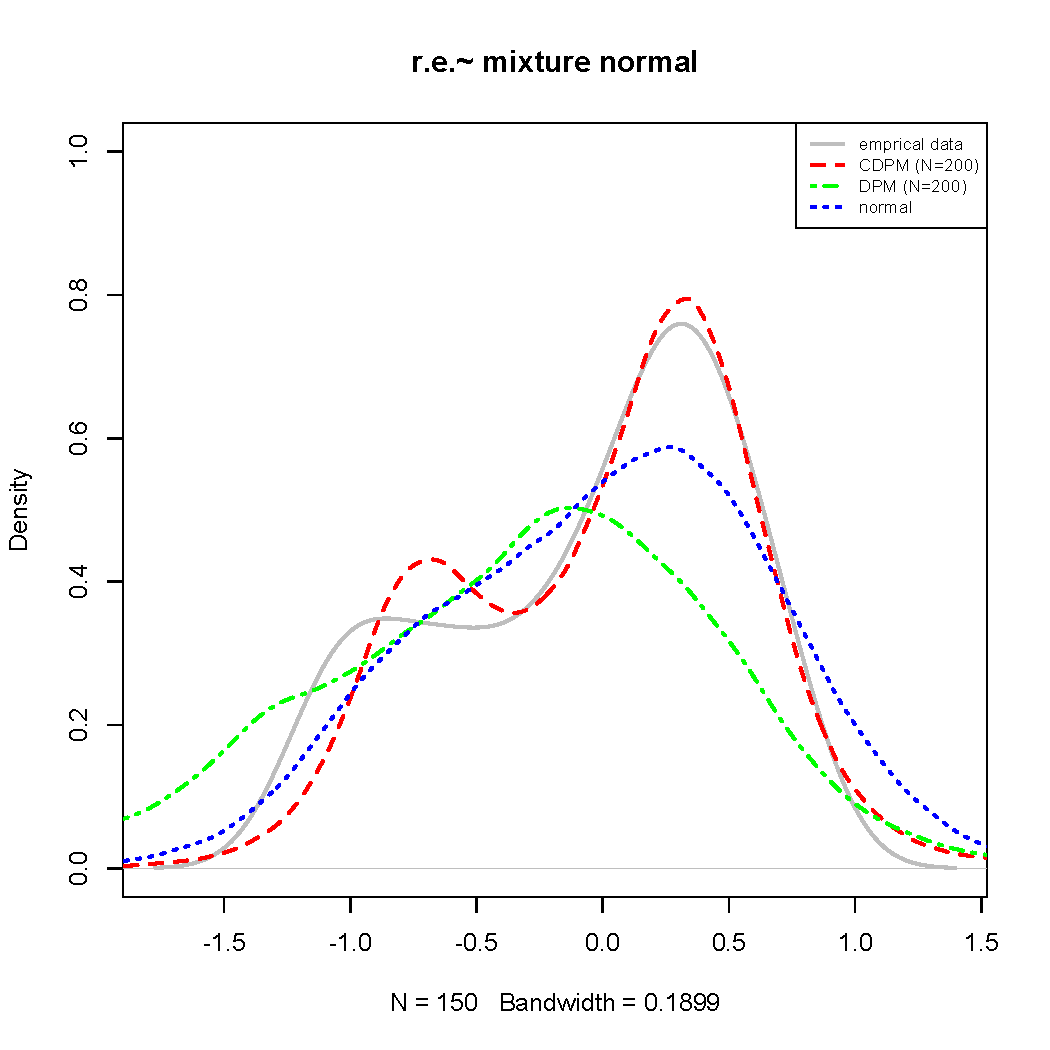
\includegraphics[width=0.85\textwidth]{ui_mixnormal.pdf}
\label{fig: normal_dpm}
\caption{\small Predicted densities of random effects that follow mixture of normals}
\end{minipage}
\begin{minipage}{0.5\textwidth}
\centering
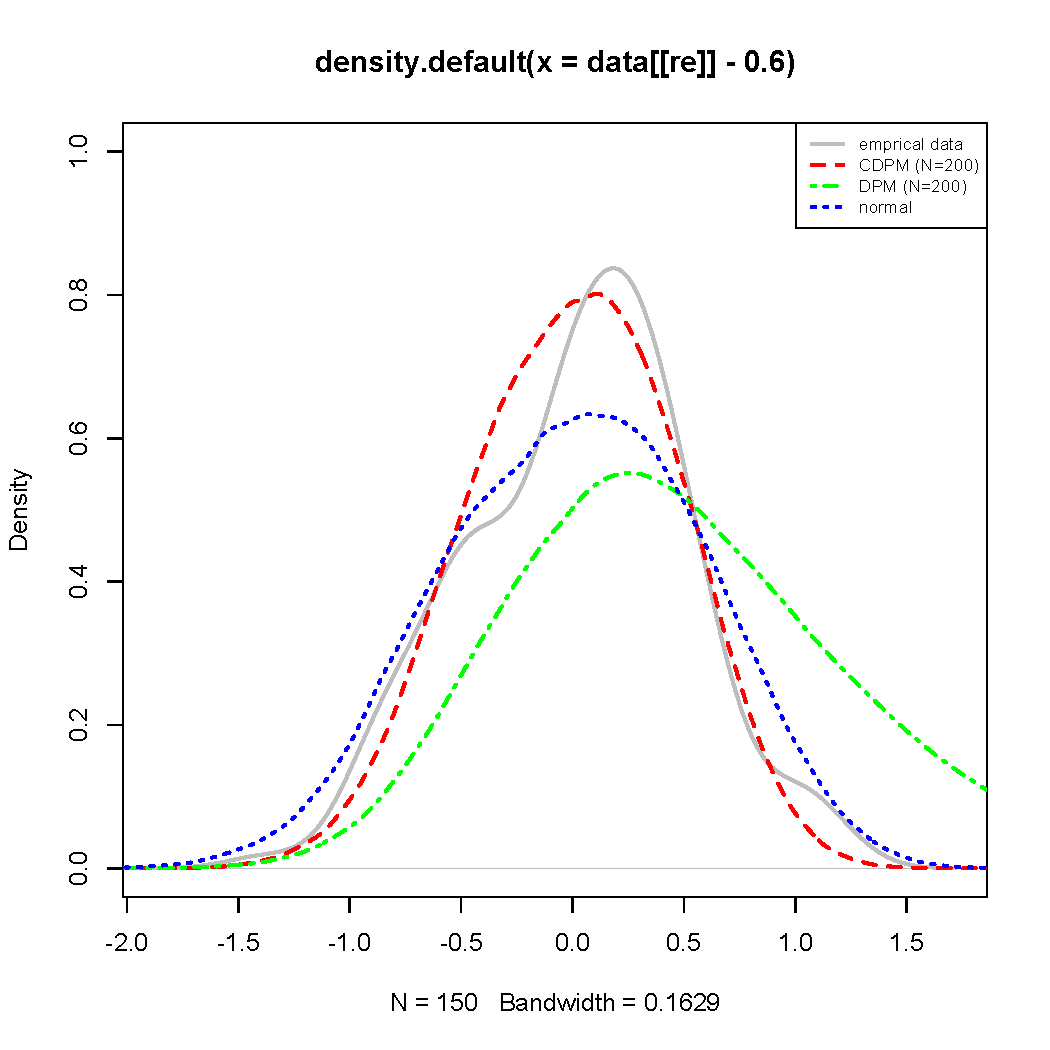
\includegraphics[width=0.85\textwidth]{ui_normal.pdf}
\label{fig: normal_dpm}
\caption{\small Predicted densities of random effects that follow $N(0.6, 0.5^2)$}
\end{minipage}
\end{figure}


\subsubsection*{Sum of squared difference}%%%%
The best predictor (BP) is defined as the one that minimize the mean squared error of the prediction \cite{mcculloch2001generalized}, that is to minimize

\begin{equation}\label{eqn:mse}
E[(\tilde{\bf u}-{\bf u})^T{\bf A}(\tilde{\bf u}-{\bf u})]=\int\int(\tilde{\bf u}-{\bf u})^T{\bf A}(\tilde{\bf u}-{\bf u})f({\bf u, y})d{\bf y}d{\bf u},
\end{equation}
where ${\bf A}$ is a positive definite symmetrical matrix.

\cite{searle2009variance} shows that the to minimize (\ref{eqn:mse}), the BP of ${\bf u}$ is given by
\begin{equation}\label{eqn:bp}
\tilde{\bf u}=E({\bf u}|{\bf y}),
\end{equation}

that is the posterior mean of the random effects ${\bf u}$. Thus, based on the result of (\ref{eqn:bp}), to compare the performance of different models in predicting the random effects,  one criteria that we can use is the sum of squared difference (SSD) between the predicted and generated random effects is calculated as follows:

\begin{equation}\label{eqn:ssd}
SSD=\sum_{i=1}^N (\tilde{u}_i-u_i)^2,
\end{equation}
where $\tilde{u}_i$ is the posterior mean of the predicted random effects for subject $i$ and the model with smaller SSD is preferred.



\subsubsection*{Posterior predictive values}%%%%
We can also sample the response variable based on the predicted distribution of the random effects, as a result, we can compare the posterior predictive values with the observed ones by using $Q-Q$ plot or relative absolute deviation (RAD) \cite{rikhtehgaran2013semi}, which is defined as

\begin{equation}\label{eqn:rad}
RAD = \sum_{i=1}^N\sum_{j=1}^{n_i}\frac{\tilde{y}_{ij}-y_{ij}}{y_{ij}}, 
\end{equation}

where $\tilde{y}_{ij}$ is the posterior predictive values sampled based on (\ref{eqn:ppv}). Similar as SSD criteria, model with smaller RAD is preferred.



\begin{table}[H]
\begin{center}
\caption{Sample summary table: statistics of prediction of random effects (RAD is based on 30 posterior samples)}
\begin{tabular}{clccc}
\hline
 & \emph{dist. of} $u_i$ & \emph{Normal} & \emph{DPM} & \emph{CDPM}\\
\hline
\multirow{3}{*}{\bf SSD} &  \emph{N(0.6, 0.25)} & 1.00 (70.52)& 0.22 (15.33)& 0.98 (69.33) \\
& \emph{beta(2,5)} & 1.00 (11.96)& 0.29 (3.50) & 0.27 (3.24)\\
& \emph{MN} &  1.00 (13.48) & 1.08 (14.56) & 0.80 (10.84)\\
\hline
\multirow{3}{*}{\bf RAD} &  \emph{N(0.6, 0.25)} & 1.00 (-2685.27)&  1.04 (-2787.77)& 1.02 (-2739.31)  \\
& \emph{beta(2,5)} & 1.00 (1939.24)& 0.81 (1563.85) & 0.84 (1634.97)\\
& \emph{MN} & 1.00 (264.39) & 0.86 (226.64)& 0.87 (228.96)\\
\hline
\end{tabular}
\end{center}
\end{table}


%\section{Results}%%%%%%%%%%%%%%%%%%%%
%\subsection{Simulation study}

%\subsection{Real data analysis}

%\section{Discussion}%%%%%%%%%%%%%%%%%%%%


%\section{Conclusion}%%%%%%%%%%%%%%%%%%%%











\bibliographystyle{plain}%%%%%%%%%%%%%%%%%%%%
\addcontentsline{toc}{section}{6 \ \ References}
\bibliography{proposal}



























\end{document}
